\documentclass[12pt, letter paper]{article}
\usepackage[utf8]{inputenc}
\title{Figure Explanations}
\author{Rasmus Raschke}
\date{March 2026}
\usepackage{amsmath} 
\usepackage{bm}
\usepackage{graphicx}
\usepackage[table,xcdraw]{xcolor} 
\usepackage{float}
\begin{document}
\section{Sketches of the System}
\begin{figure}[H]
    \centering
    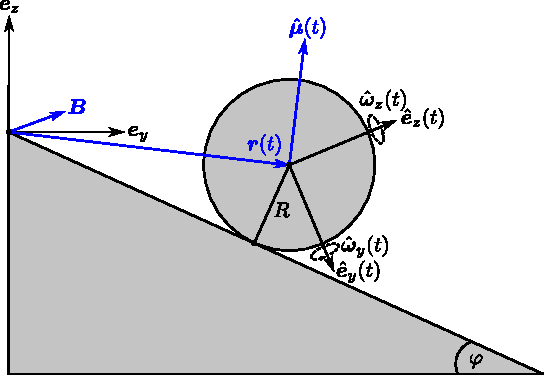
\includegraphics[width=\linewidth]{ramp.pdf}
    \caption{Depicted is the $yz$-projection of the incline system, the $z$-direction is orthogonal to the paper plane. The incline has an inclination angle $\varphi$ and the sphere is of radius $R$. Two orthonormal coordinate frames are considered: The fixed frame $\{ \bm{e}_x, \bm{e}_y, \bm{e}_z\}$ and the body frame $\{ \hat{\bm{e}}_x, \hat{\bm{e}}_y, \hat{\bm{e}}_z \}$. Vectors expressed in the body frame carry hats and are time-dependent, stationary vectors not. Blue vectors might have a non-zero $z$-component and are therefore only projections. The outer magnetic field is represented by $\bm{B}$, the magnetic dipole vector of the sphere by $\hat{\bm{\mu}}(t)$, and the centre of mass measured from the fixed frame by $\bm{r}(t)$. The in-plane angular velocities of the body frame are shown as $\hat{\bm{\omega}}_x$ and $\hat{\bm{\omega}}_y$.}
    \label{fig:ramp}
\end{figure}
\begin{figure}[H]
    \centering
    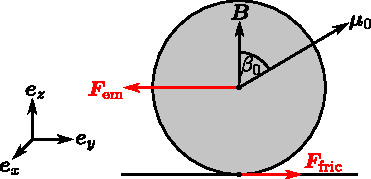
\includegraphics[width=\linewidth]{flat.pdf}
    \caption{Shown is a sketch of the flat system with sufficiently small initial displacement angle $\beta_0$ between the outer magnetic field $\bm{B}$ and the initial magnetic dipole vector $\bm{\mu}_0$. Note that the system is effectively reduced to two dimensions. The red vectors indicate the oscillation-driving electromagnetic force $\bm{F}_\text{em}$ and the damping frictional force $\bm{F}_\text{fric}$. The frictional force includes aerodynamical drag and rolling resistance.}
    \label{fig:flat}
\end{figure}
\section{Figure Family A}
These figures are results of a proof-of-concept toy model: The incline without electromagnetic interaction. The goal is to compare numerical results to analytical equations.
\renewcommand{\thefigure}{A1}
    \begin{figure}[H]
        \centering
        
\includegraphics[width=\linewidth]{FIGA1_no_mag_traj.pdf}
        \caption{Shown are different evolutions of the $y$-projection of the centre-of-mass coordinate $\bm{r}=(x,y,z)^\top$ over time $t$ for different incline angles $\varphi$ without friction. Lines were calculated from the analytical solution and compared to the numerical results, represented as dots.}
    \end{figure}
\renewcommand{\thefigure}{A2/A3}
    \begin{figure}[H]
        \centering
        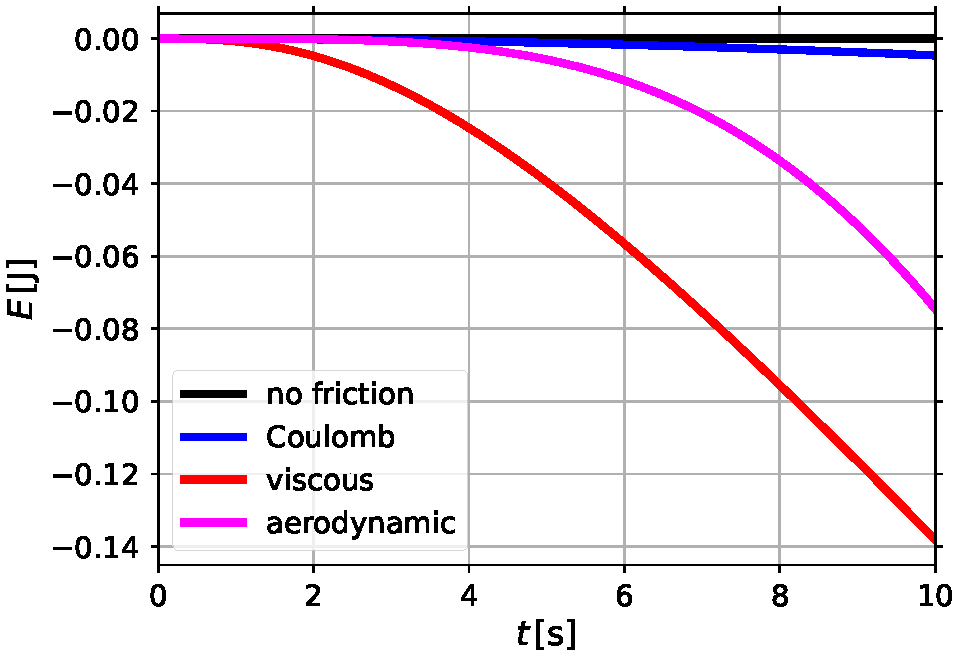
\includegraphics[width=0.45\linewidth]{FIGA2_no_mag_fric_energ.pdf}
        
\includegraphics[width=0.45\linewidth]{FIGA3_no_mag_fric_traj.pdf}
        \caption{The left plot shows the energy evolution $E(t)$ of the system over time $t$, while the right one depicts the $y$-COM-coordinate evolution. The data originates from the numerical simulation program. Compared are different friction models, where \emph{Coulomb} represents dry rolling resistance, \emph{viscous} represents a linear damping approximation to rolling resistance, and \emph{aerodynamic} represents spherical aerodynamic drag.}
    \end{figure}
\section{Figure Family B}

\section{Figure Family C}

\section{Figure Family D}

\section{Figure Family E}


\end{document}
